\documentclass{article}
\usepackage{blindtext}
\usepackage[utf8]{inputenc}
\usepackage{amsmath,bm}
\usepackage{amstext}
\usepackage{amsfonts}
\usepackage{amsmath}
\usepackage{multirow}
\usepackage{enumerate}
\usepackage{xeCJK}
\setCJKmainfont{STKaiti}
\usepackage[noend]{algpseudocode}
\usepackage{algorithmicx,algorithm}
 \usepackage{graphicx}
 \usepackage{float}
\usepackage{listings}
\lstset{
	columns=fixed,       
	numbers=left,                                        % 在左侧显示行号
	numberstyle=\tiny\color{gray},                       % 设定行号格式
	frame=none,                                          % 不显示背景边框
	keywordstyle=\color[RGB]{40,40,255},                 % 设定关键字颜色
	numberstyle=\footnotesize\color{darkgray},           
	commentstyle=\it\color[RGB]{0,96,96},                % 设置代码注释的格式
	stringstyle=\rmfamily\slshape\color[RGB]{128,0,0},   % 设置字符串格式
	showstringspaces=false,                              % 不显示字符串中的空格
	language=matlab,                                        % 设置语言
}

\title{矩阵论及其应用实习题}
\author{陈轶洲 MF20330010}
\begin{document}
	\maketitle
	\numberwithin{equation}{section}
	
\section{实验环境}

计算机型号:MacBook Air \\
操作系统:Mac os\\
编程语言:Matlab
	
	
\section{CPU时间}
输入第一组数据:$ K=8,M=50,N=100 $\\
由于数据规模不大,所以该算法消耗的CPU时间只有几毫秒\\
\begin{figure}[h]
	\centering
	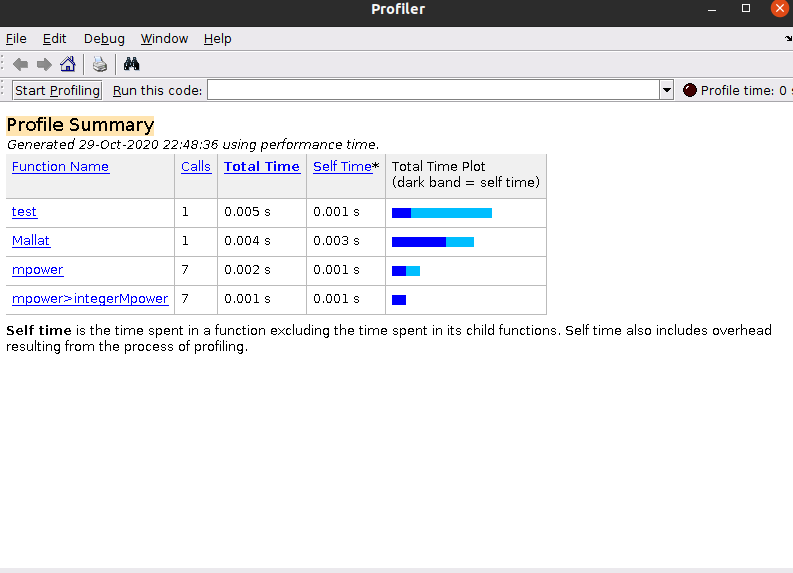
\includegraphics[scale=0.6]{test1.png}
\end{figure}

输入第二组数据:$ K=1000,M=15000,N=23000 $\\
第二组数据规模远远超过第一组,耗时332.012s
\begin{figure}[h]
	\centering
	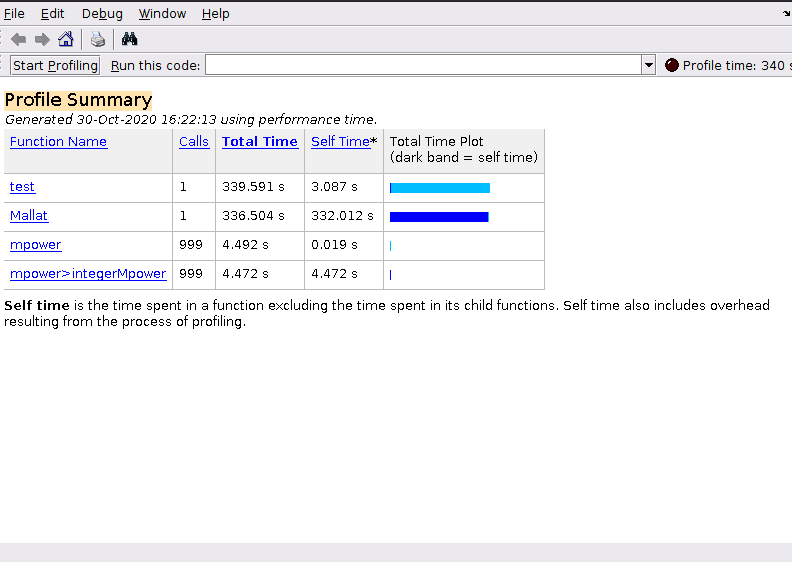
\includegraphics[scale=0.6]{test2.png}
\end{figure}

\section{算法说明}
\subsection{算法步骤}
	\begin{algorithm}[H]
		\caption{正交匹配追踪算法$ Mallat(y,A,K) $} 
		\hspace*{0.02in} {\bf Input:} 
		观测数据向量$ y\in R^{M\times 1},$ 字典矩阵 $ A \in R^{M\times N},$ 稀疏性指标 $K\in N$\\
		\hspace*{0.02in} {\bf Output:} 
		稀疏的信号向量$ x \in R^{N\times 1}$ 
		\begin{algorithmic}[1]
			\State 初始化:$ \Omega_0=\phi,r_0=y,k=1 $ 
			\While{$ k\leq K $} 
			\State $ j_k\in \arg{\max_j{|(r_{k-1},a_j)|}} $
			\State $ \Omega_k = \Omega_{k-1}\cup \{j_k\} $
			\State $ x_k = (A_{\Omega_k}^{T}A_{\Omega_k})^{-1}A_{\Omega_k}^{T}y $
			\State $ r_k = y-A_{\Omega_k}x_k $
			\State $ k += 1 $
			\EndWhile
			\State $  \hat{x}(i) = \left\{
			\begin{aligned}
				x_K(i) \qquad i\in \Omega_K\\
				0 \qquad others
			\end{aligned} 
			\right. $
			\State \Return $ \hat{x} $
		\end{algorithmic}
	\end{algorithm}
\subsection{变量说明}
使用Matlab设计的正交匹配追踪算法中,对变量做如下定义:\\
1.A为测度矩阵,规模为$ M\times N $;\\
2.x为待重构向量,规模为$ N\times 1 $;\\
3.y为观测所得向量,规模为$ M\times 1 $;\\
4.K为稀疏性指标,为正整数;\\
5.r为残差向量,规模为$ M\times 1 $;\\
6.At,每轮迭代时被选中的列;\\
7.$ x_l $为最小二乘解;\\
8.$ x_r $为经过算法重构的向量。

\subsection{程序清单}
首先在Mallat.m中实现正交匹配追踪算法:
\begin{lstlisting}
function [ x ] = Mallat(y,A,K)
	[M,N] = size(A);%字典矩阵的规模
	x = zeros(N, 1);%需要重构的解向量x
	At = zeros(M, K);%存储每轮迭代时A中被选中的列
	x_pos = zeros(1, K);%存储每轮迭代时A中被选中列的序号
	r = y;%残差向量,初始化为y
	
	for ii = 1:K%迭代K轮
		product = A'*r;%计算矩阵各列与残差的点积
		[val, pos] = max(abs(product));%找到与残差最相关的列
		At(:,ii) = A(:,pos);%将被选中的列存储到At中
		x_pos(ii) = pos;%记录被选中列的序号
		A(:,pos) = zeros(M,1);
		x_l = (At(:,1:ii)'*At(:,1:ii))^(-1)*At(:,1:ii)'*y;%最小二乘解
		r = y - At(:,1:ii)*x_l;%更新残差
	end
	
	x(x_pos) = x_l;
end
\end{lstlisting}
接着在test.m中对两组规模的数据进行测试
\begin{lstlisting}
	K=8;
	M=50;
	N=100;
	A=randn(M,N);
	x=randn(N,1);
	kk=randperm(N);
	x(kk(1:N-K))=0;
	y=A*x;
	x_r1 = Mallat(y,A,K);
	stem([x,x_r1]);
	
	K=1000;
	M=15000;
	N=23000;
	A=randn(M,N);
	x=randn(N,1);
	kk=randperm(N);
	x(kk(1:N-K))=0;
	y=A*x;
	x_r2 = Mallat(y,A,K);
	stem([x,x_r2]);
\end{lstlisting}

\section{运行结果及分析}
\subsection{$ K=8,M=50,N=100 $}
以第一组数据为例,当$ M=50,N=100 $时,取稀疏性系数$ K=8 $,通过随机生成的系数向量$ x $生成观测所得向量,并通过正交匹配追踪算法得到重构向量$ x_r $,其输出如下:\\
$ x $:\\
\begin{figure}[H]
	\centering
	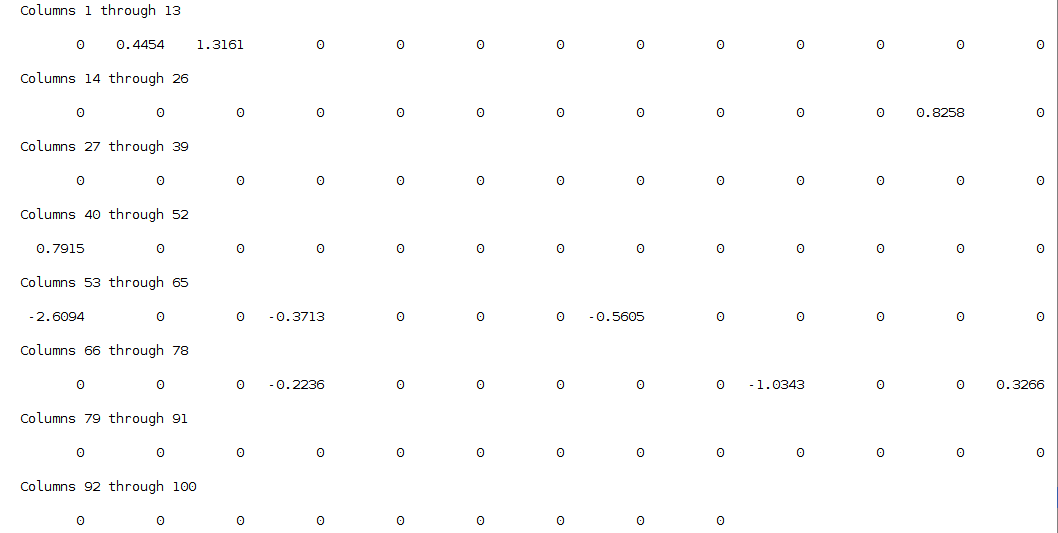
\includegraphics[scale=0.6]{x.png}
\end{figure}
$ x_r $:
\begin{figure}[H]
	\centering
	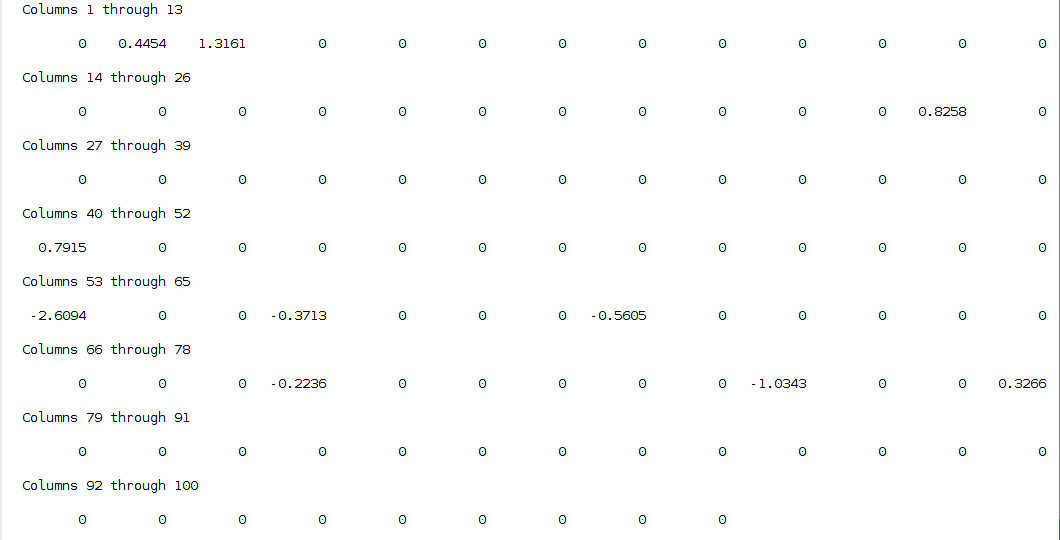
\includegraphics[scale=0.6]{x_r.png}
\end{figure}

通过matlab自带的绘图函数stem()绘制两个向量的针状图
\begin{figure}[H]
	\centering
	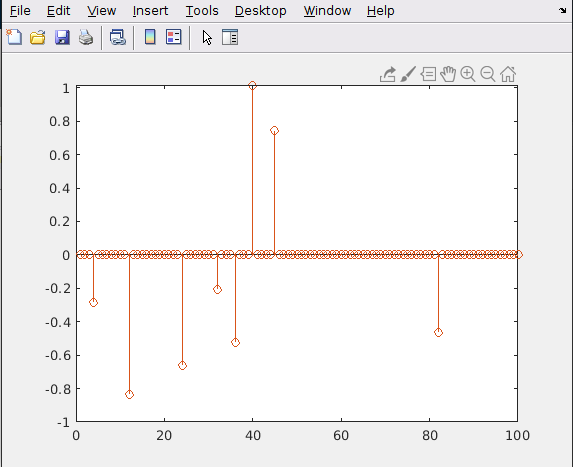
\includegraphics[scale=0.6]{k8.png}
\end{figure}
结合输出向量和图表可知重构向量与原始向量相同,在该条件下正交匹配追踪算法能根据观测向量完美重构向量

\subsection{$ K=12,M=50,N=100 $}
仍使用第一组数据,将稀疏性系数$ K $增大到12,由图可知重构向量与原向量几乎没有误差
\begin{figure}[H]
	\centering
	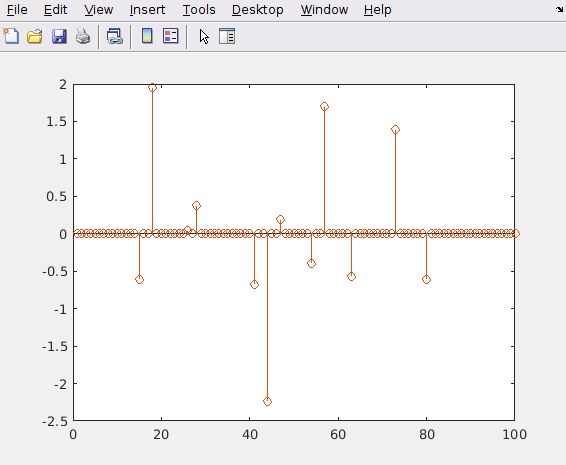
\includegraphics[scale=0.6]{k12.png}
\end{figure}

\subsection{$ K=16,M=50,N=100 $}
将稀疏性系数$ K $继续增大到16,由图可知此时重构向量与原向量之间出现误差
\begin{figure}[H]
	\centering
	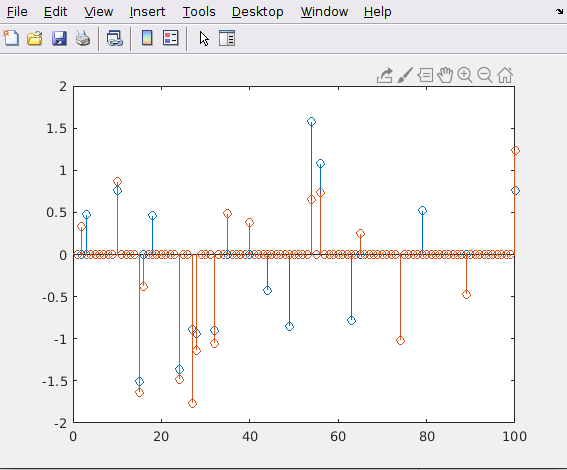
\includegraphics[scale=0.6]{k16.png}
\end{figure}

\subsection{$ K=24,M=50,N=100 $}
当稀疏性系数$ K $继续增大到24后,重构向量与原向量之间的误差进一步增大
\begin{figure}[H]
	\centering
	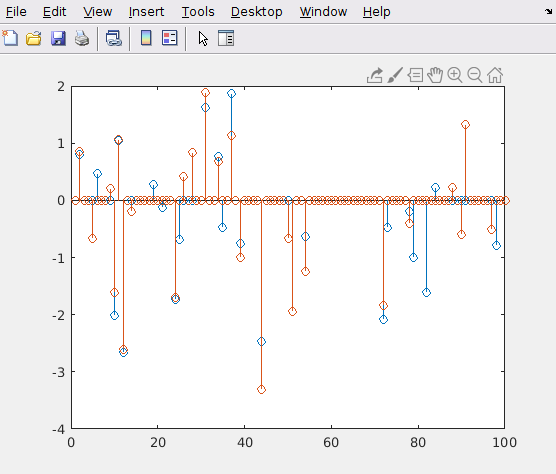
\includegraphics[scale=0.6]{k24.png}
\end{figure}

\subsection{$ K=1000,M=15000,N=23000 $}
考虑第二组数据,由图可知重构向量与原向量几乎没有误差
\begin{figure}[H]
	\centering
	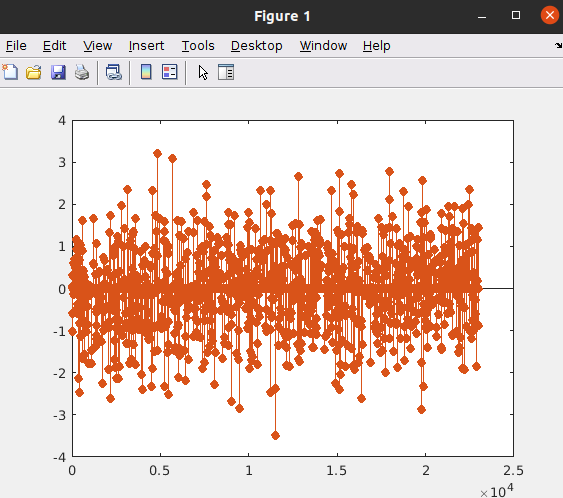
\includegraphics[scale=0.6]{k1000.png}
\end{figure}

\subsection{结果分析}
\begin{enumerate}[1)]
	\item 对于两组输入数据,分析其CPU运行时间,可以发现:对于小规模输入,正交匹配追踪算法可以在几毫秒内求出结果;而对稍大规模数据,该算法的求解效率依然很可观;
	\item 根据第一组实验,在确定M和N后,K的取值决定了最后重构向量的表现:$ K<<N $时重构向量与原向量几乎无误差,而随着K的增大,重构向量与原向量之间的误差也越来越大,根据文献$ [1] $可以看出信号稀疏度K与重构成功概率之间的关系:
	\begin{figure}[H]
		\centering
		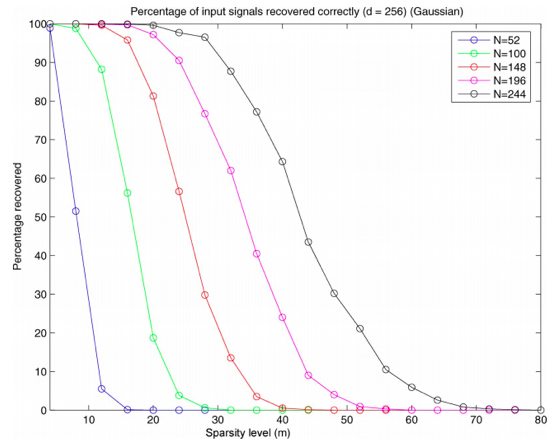
\includegraphics[scale=0.6]{1.png}
	\end{figure}
\end{enumerate}

\section{实验总结}
\begin{enumerate}[1)]
	\item 通过计算程序运行CPU时间可以发现,正交匹配追踪算法的时间复杂度并不高,这是由于它本质上是一个贪心算法,通过稀疏性系数K来决定迭代次数,这样就避免了对整个系数矩阵进行求逆等耗时的操作;
	\item 在进行算法设计过程中,我考虑利用残差向量寻找到A中与其内积绝对值最大的列后,将该列置为零。后来发现这一步是不必要的,因为在之后的轮次中,残差向量与该列正交,所以不会出现重复选择某一列的情况;
	\item 对于“增大稀疏性系数K后误差变大”这一现象,我认为可以类比主成分分析(principal component analysis, PCA),正交匹配算法每轮选择与残差向量内积绝对值最大的列,可以认为这些列最大程度地保留了向量的信息,而随着K的增大,所选择的列越多,这样势必会加入一些与向量相关性不大的列,从而给信号带来噪声,使得重构误差增加。	
\end{enumerate}

\section{参考文献}
	$ [1] $ Joel A. Tropp and Anna C. Gilbert. Signal Recovery From Random Measurements Via Orthogonal Matching Pursuit[J]. IEEETransactions on Information Theory, VOL. 53, NO. 12, DECEMBER 2007.

\end{document}
